\part*{Annexes}
\appendix

\subsection*{Documents complémentaires}
\begin{figure}[H]
    {\centering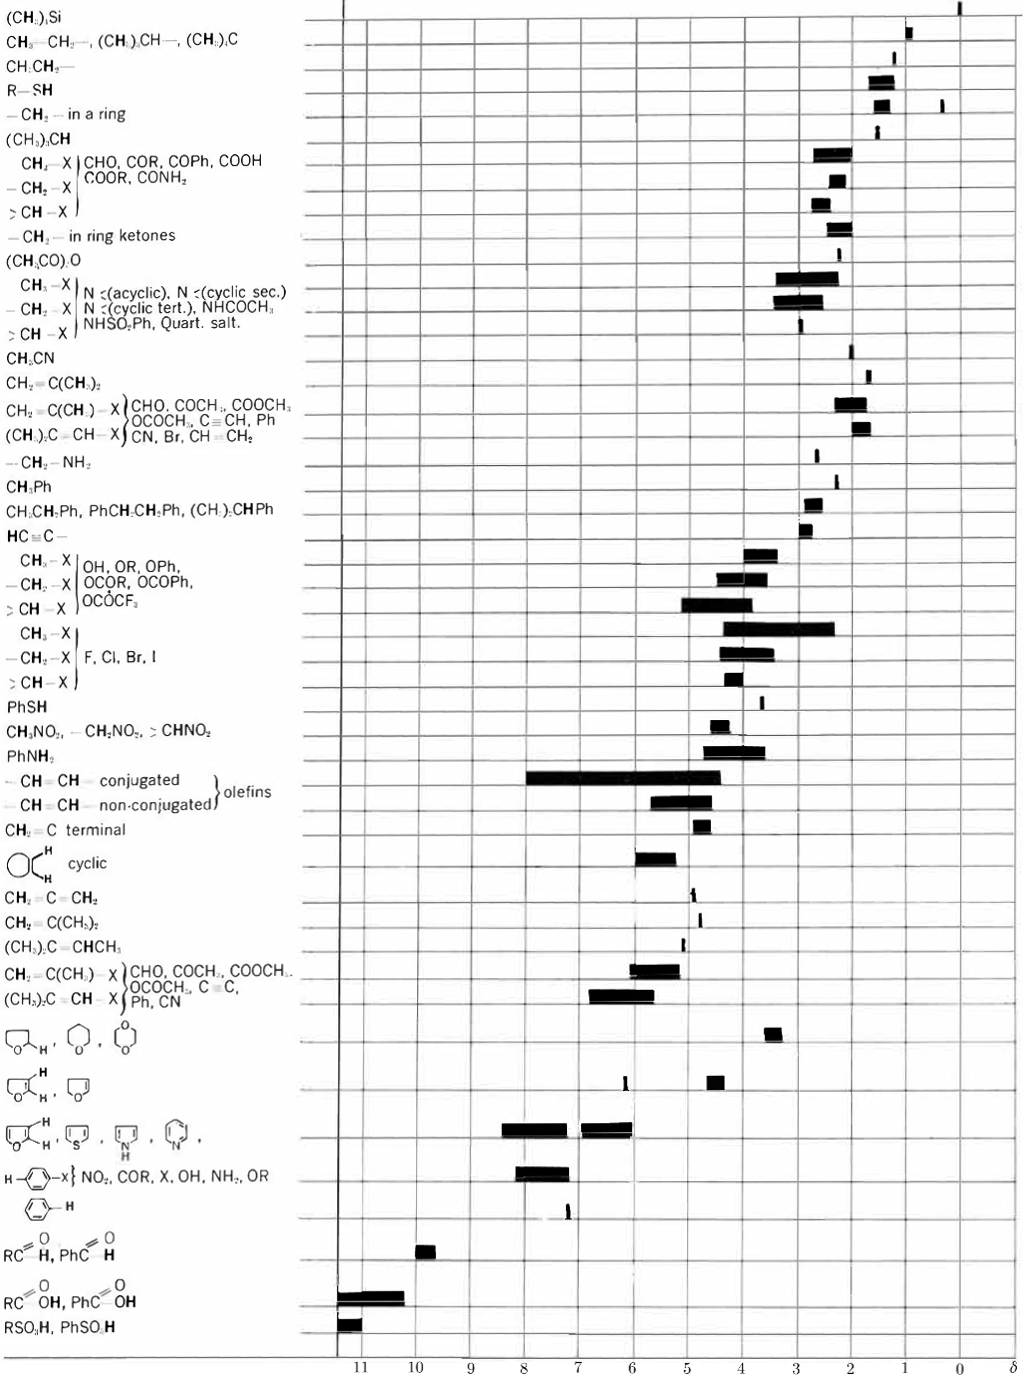
\includegraphics[width=\linewidth]{chimiePC/misc/RMN.png}}
    Déplacements chimiques caractéristiques en RMN du proton $^{1}$H pour des structures organiques usuelles d'après E. Mohacsi, \emph{J. Chem. Educ.} 1964, \textbf{41}, 1, 38.
\end{figure}

\begin{figure}[H]
    {\centering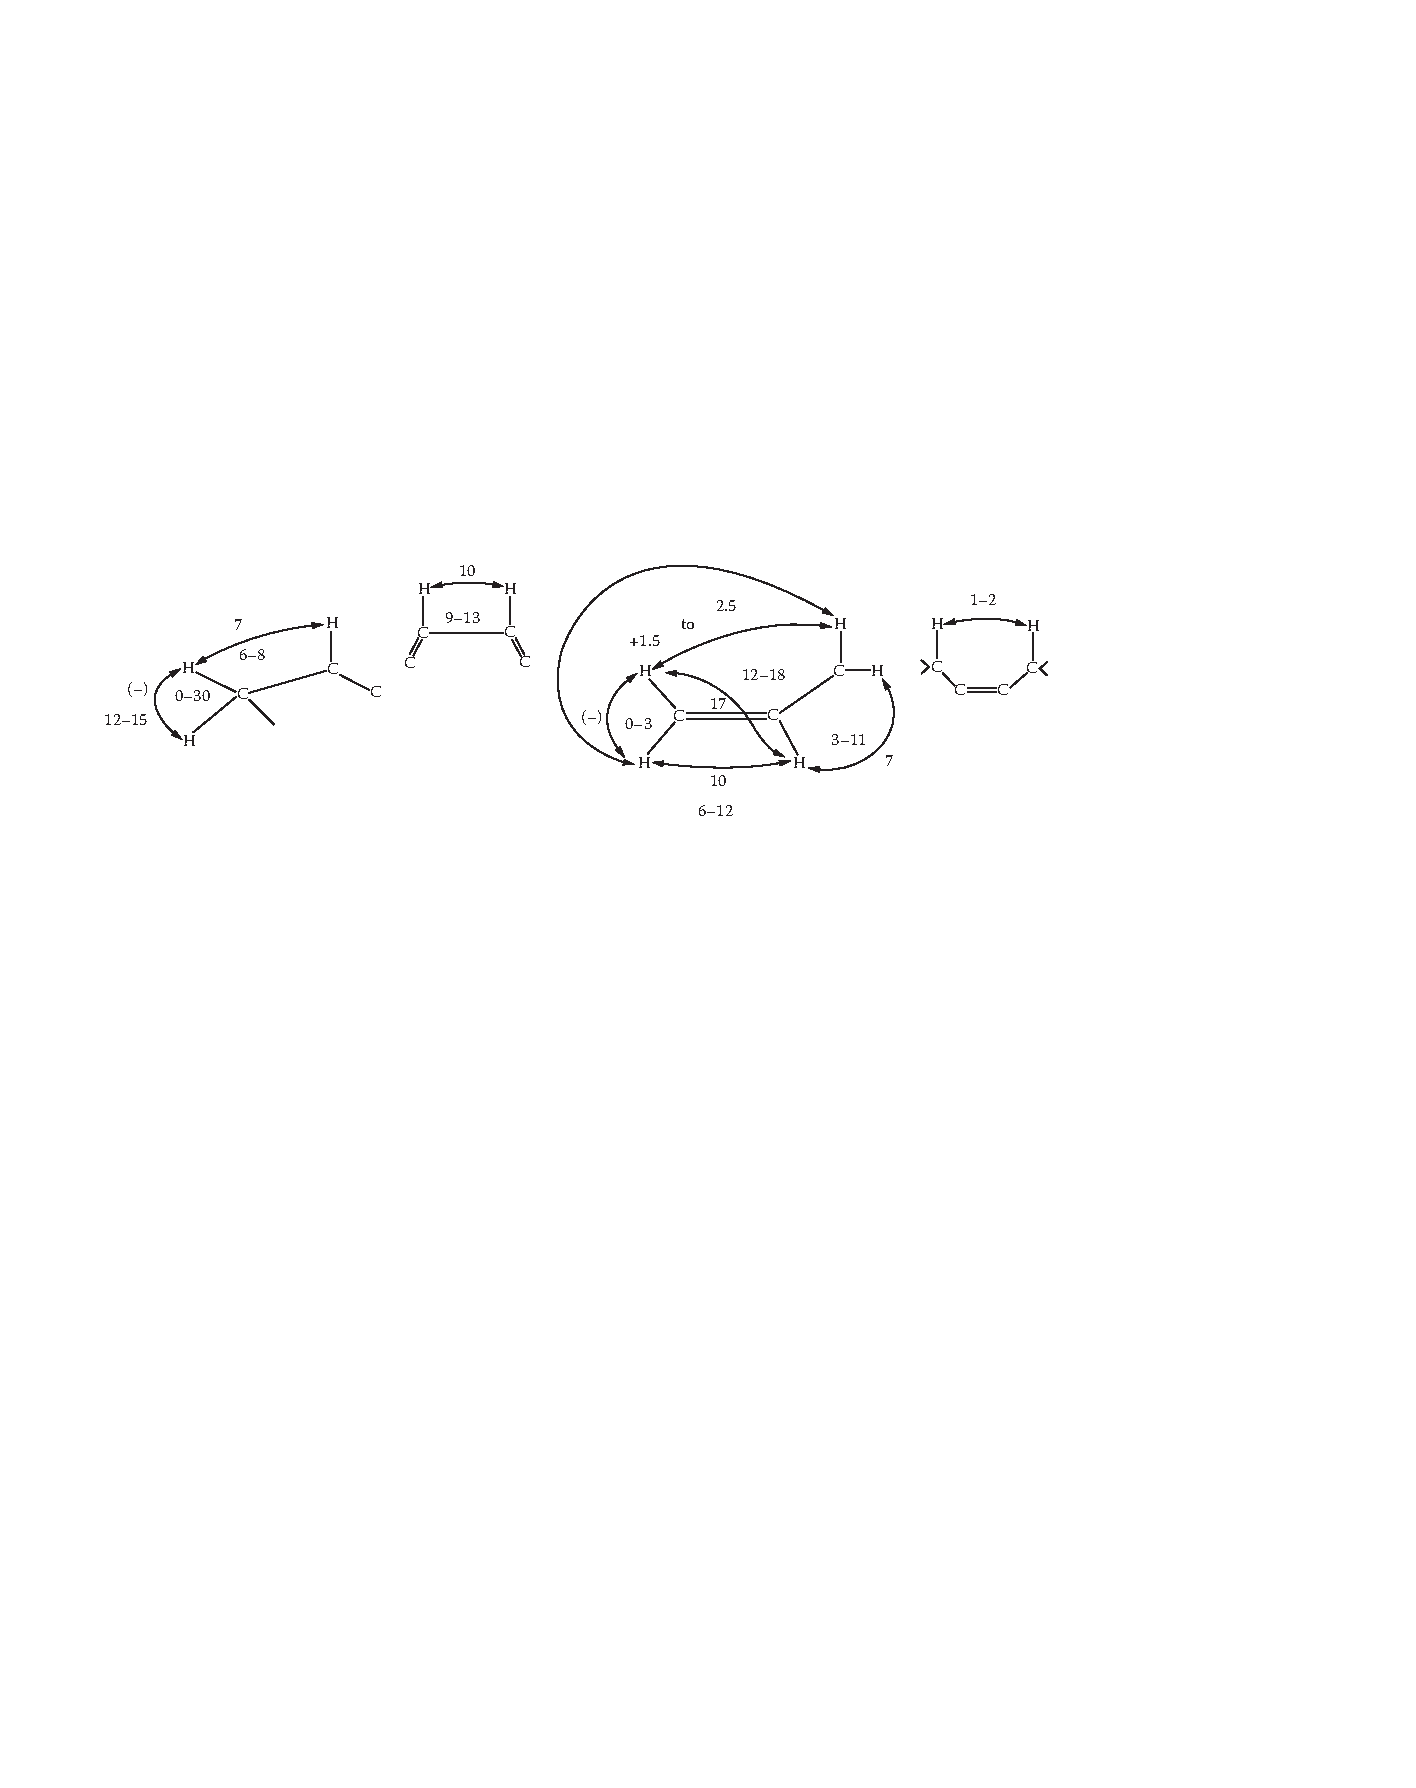
\includegraphics[width=\linewidth]{chimiePC/misc/RMN-J1.pdf}}
    Constantes de couplage $J$ caractéristiques en RMN du proton $^{1}$H pour les alcanes et les alcènes \\ d'après \emph{CRC Handbook of chemistry}, 97ème ed.
\end{figure}

\subsection*{Idées en vrac}
\begin{itemize}
    \item MECA
    \begin{itemize}
        \item le camion dans un virage : va-t-il glisser ? / le train : va-t-il verser ?
        \item ondes gravitationnelles
        \item taille de ma fiat 500 après un contresens sur l'A10 ?
    \end{itemize}
    \item MECAFLU
    \begin{itemize}
        \item STATIQUE
        \begin{itemize}
            \item surface libre d'un liquide en rotation
            \item surface libre d'un liquide dans un camion citerne : quand ça déborde ?
            \item camion citerne : va-t-il verser ? Quelle différence avec le cas solide ?
            \item fréquence de Brunt-Vasila
            \item altitude idéale pour le vol Flybe Manchester--Aberdeen ? (réponse : 1m du sol pour qu'il s'écrase)
        \end{itemize}
        \item Torricelli, vidage d'une baignoire puis vidage d'un jerrican (cf exo jerrican en statique des fluides)
        \item instabilité de Rayleigh--Taylor.
        \item décrire le comportement d'un filet d'eau : il passe d'un régime laminaire à déperlant (instabilité de Rayleigh--Plateau,  cf X 2016 physique B partie 2, c'est atroce)
        \item je lance un objet de densité $d$ dans l'eau depuis une hauteur $H$. A quelle condition l'objet rentre dans l'eau ? A quelle condition l'objet remonte à la surface ?
        \item Cellule hele-shaw (stage gérgoire <3), loi de Darcy
        \item \emph{Jardins sous la pluie}
            
    \end{itemize}
    \item THERMO
    \begin{itemize}
        \item laisser le frigo ouvert
    \end{itemize}
    \item ELECTROMAG
    \begin{itemize}
        \item railgun
    \end{itemize}
    \item OPTIQUE
    \begin{itemize}
        \item combien de centrales nucléaires faut-il pour faire fonctionner le sabre laser de Luc Skywalker ?
    \end{itemize}
    \item QUANTIQUE
    \item ODG RIGOLOS
    \begin{itemize}
        \item proportion en eau de la vache
        \item combien de grains de sable dans une baignoire
        \item combien de couches de graphites lorsqu'on écrit avec un crayon à papier
    \end{itemize}
    
    \item Filtre passe-bande à pont de wien ($Q = 1/3$)
\end{itemize}

\nocite{*}
\printbibliography